\section{Minimal stretch factors for non-orientable surfaces with marked points}
\label{sec:application}

In this section we will use \autoref{thm:classifying-fibrations} and Proposition  \ref{prop:asymptotic} to adapt the methods of Yazdi \cite{yazdi2018pseudo} to non-orientable surfaces. We recall the statement of the main theorem:
\begin{manualtheorem}
  {\ref{thm:stretch1}}
Let $\no_{g,n}$ be a non-orientable surface of genus $g$ with $n$ punctures, and let $\ell_{g,n}'$ be the logarithm of
  the minimum stretch factor of the pseudo-Anosov mapping classes acting on $\no_{g,n}$.
  Then for any fixed $n \in \mathbb{N}$, there is a positive constant $B'_1 = B'_1(n)$ and $B'_2 = B'_2(n)$ such
  that for any $g \geq 3$,
  the quantity $\ell_{g,n}'$ satisfies the following inequalities:
  \begin{align*}
    \frac{B'_1}{g} \leq \ell'_{g,n} \leq \frac{B'_2}{g}.
  \end{align*}
\end{manualtheorem}





Observe that the lower bound for the non-orientable case follows easily from the lower bound for the orientable case.
Indeed, let $\varphi$ be a pseudo-Anosov map with the minimal stretch factor on $\no_{g,n}$. The orientation double cover of $\no_{g,n}$ is $\os_{G,2n}$, where $G = g-1$.  Note that in the non-orientable case we measure genus as the number of copies of the projective plane attached to $S^2$ via a connect sum and in the orientable case we measure genus as the number of copies of the torus attached to $S^2$ via a connected sum. Let $\wt{\varphi}:\os_{G, 2n}\to\os_{G,2n}$ be the orientation preserving lift of $\varphi$.
By Proposition \ref{prop:2}, $\wt{\varphi}$ has the same
stretch factor as $\varphi$. The logarithm of the former is bounded below by $\frac{B_1}{G}$ (where $B_1$ is given by Yazdi \cite{yazdi2018pseudo}), and thus the stretch factor of $\varphi$ is bounded
below as well. The more challenging part of the proof is showing that the upper bound holds. 

We will closely follow Yazdi's construction, which proceeds in five steps, though we will reorder them for clarity.  In steps 1 and 2, we construct a family of psuedo-Anosov homeomorphisms
of $\no_{g_i,n}$, where $\{g_i\}$ is an unbounded increasing sequence. However the sequence $\{g_i\}$ does not contain all natural numbers.  In step 3 we give an upper bound to the stretch factor of the previously constructed homeomorphisms. In steps 4 and 5, we construct pseudo-Anosov maps on surfaces of genera that do not belong to the sequence $\{g_i\}$. It is in steps 4 and 5 that we uses
Thurston's fibered face theory. We have adapted  each of Yazdi's five steps to work for non-orientable surfaces.

\p{Step 1: Constructing the surfaces}


We begin by defining a family of surfaces $P_{n,k}$. Let $S$ be an orientable surface of genus 5 with 3
boundary components.  Call the boundary components $c,d$ and $e$. Choose an orientation of $S$ and let $c,d$ and $e$ inherit the induced orientations. Let $p$ and $q$ be marked points in the boundary component $e$. In Step 5 we will remove $p$ and all its copies.  Let  $r$ and
$s$ be the components of $e\setminus\{p,q\}$. We obtain a non-orientable surface $T$ from $S$ by adding two cross caps to $S$ (retaining the orientation of the boundary components of $S$).  The resulting surface $T$ is shown in \autoref{fig:buildingblock}.

\begin{figure}[ht]
    \centering
    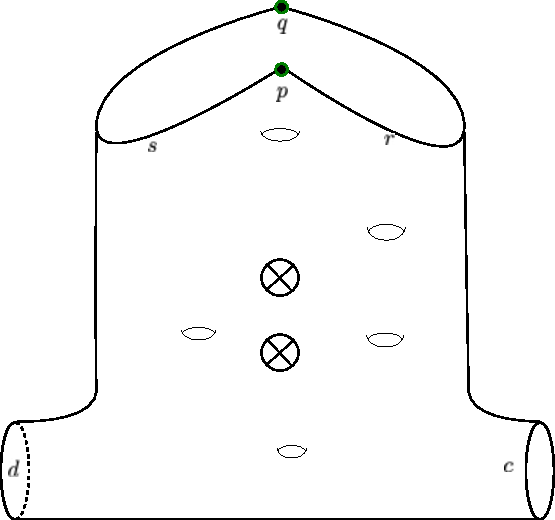
\includegraphics[scale=0.8]{t.pdf}
    \caption{The surface $T$, which will be the building block of the construction.}
    \label{fig:buildingblock}
\end{figure}

Let $T_{i,j}$ be copies of the surface $T$, where $i,j \in \mathbb{Z}$. Let $c_{i,j}, d_{i,j}$ and $e_{i,j}$ be the (oriented) boundary components of $T_{i,j}$ and let $r_{i,j}$ and $s_{i,j}$ be the copies of the arcs $r$ and $s$ in $T_{i,j}$. Define a connected infinite surface $T_\infty$ as the quotient:
\begin{align*}
  T_\infty \coloneqq \left. \left( \bigcup T_{i,j} \right)\right/\sim
\end{align*}
for all integers $i$ and $j$. The gluing $\sim$ is given by orientation-reversing identifications:
\begin{align}
  c_{i,j} &\sim d_{i+1,j} \label{identification1}\\
  r_{i,j} &\sim s_{i,j+1}.\label{identification2}
\end{align}

We have two
natural shift maps $\overline{\rho_1},\overline{\rho_2}: T_\infty \to T_\infty$ that act in the
following manner:
\begin{align*}
  \overline{\rho_1}: T_{i,j} &\mapsto T_{i+1, j} \\
  \overline{\rho_2}: T_{i,j} &\mapsto T_{i, j+1}.
\end{align*}

Note that $\overline{\rho_1}$ and $\overline{\rho_2}$ commute. Define the surface $P_{n,k}$ as the quotient of the surface $T_\infty$ by the
covering action of the group generated by $(\overline{\rho_1})^n$ and $(\overline{\rho_2})^k$. Then
$\overline{\rho_1}$ and $\overline{\rho_2}$ are equivariant with respect to the covering map.  We denote the induced homeomorphisms of the quotient $P_{n,k}$ by $\rho_1$
and $\rho_2$.  Note that later we will require that $k\geq 3$ and $n$ is the number of punctures, given in \autoref{thm:stretch1}.

\begin{lem}
\label{lem:genera}
Let
\begin{align*}
    g_{n,k} &= (14k - 2)n + 2
\end{align*} for $n \geq 1$ and $k \geq 1$.
    The genus of $P_{n,k}$ is $g_{n,k}$.
\end{lem}
\begin{proof}
  Let $U \subset P_{n,k}$ be the subsurface
  \begin{align*}
    U = \left. \left( \bigcup_{j =0}^{k-1} T_{0,j} \right)\right/\sim'
  \end{align*}
  where $\sim'$ is given by (\ref{identification1}) and (\ref{identification2}) and by identifying $r_{i,k-1}$ and $s_{i,0}$.
  Then $U$ is a compact, non-orientable surface of genus $12k$ with $2k$ boundary components. 
  The surface $P_{n,k}$ consists of $n$ copies of $U$ identified along the $2k$ boundary components.  Therefore the Euler characteristic of $P_{n,k}$ is:
  \begin{align*}
    \chi(P_{n,k}) &= n \cdot \chi(U)\\
                  &=n\cdot(2-12k-2k)\\
                  &= -n(14k - 2).
  \end{align*}
  Since $P_{n,k}$ is a non-orientable surface with empty boundary, we have that:
  \begin{equation*}
    g_{n,k} = n(14k-2) + 2. \qedhere
  \end{equation*}
\end{proof}

\p{Step 2: Constructing the maps}
In what is now a classical paper, Penner gives a construction of pseudo-Anosov homeomorphisms on both orientable and non-orientable surfaces \cite{penner1988construction}.  Below we outline the Penner construction for non-orientable surfaces following the details of Liechti--Strenner \cite[Section 2]{LS}.



 \p{Inconsistent markings} Let $\no$ be a non-orientable surface and let $c$ be a two-sided curve in $\no$.  There exists a neighborhood of $c$ that is homeomorphic to an annulus.  Let $\mathcal{A}_c$ be an annulus and let $\zeta_c: \mathcal{A}_c \xrightarrow{} \no$ be the homeomorphism that maps to a neighborhood of $c$.  The homeomorphism $\zeta_c$ is called a \textit{marking} of $c$. A pair consisting of a curve $c$ and $\zeta_c$ is called a {\it marked curve}.
 If we fix an
orientation of $\mathcal{A}_c$, then we can pushforward this orientation to $\no$. Let
$(c,\zeta_c)$ and $(d,\zeta_d)$ be two marked curves that intersect at one point $p$.  We say that $(c,\zeta_c)$ and $(d,\zeta_d)$ are {\it marked inconsistently} if the
pushforward of the orientation of $\mathcal{A}_c$ disagrees with the pushforward of the orientation of $\mathcal{A}_d$ in a neighborhood of $p$.  We emphasize that we can also say that two disjoint curves are inconsistently marked.

\p{Dehn twists} We define the Dehn twist $\phi_{c,\zeta_c}(x)$ around a marked curve $(c,\zeta_c)$ as:
\begin{align*}
  \phi_{c,\zeta_c}(x) =
  \begin{cases}
    \zeta_c \circ \tau_c \circ \zeta_c^{-1}(x) & \text{for } x \in \zeta_c(\mathcal{A}_c) \\
    x & \text{for } x \in \no - \zeta_c(\mathcal{A}_c)
  \end{cases}.
\end{align*}
Here $\tau_c$ is the left-handed Dehn twist on $\mathcal{A}_c$, i.e. $\tau_c(\theta,t) = (\theta + 2\pi t,t)$.

\p{The Penner construction for non-orientable surfaces} Let $\mathcal{C}$ be a set of marked essential simple closed curves in $\no$ such that no two curves in $\mathcal{C}$ are homotopic.  A Penner construction on $\no$ is a composition of Dehn twists about the marked curves in $\mathcal{C}$ such that:
\begin{enumerate}
\item the complement of curves in $\mathcal{C}$ in $\no$ consists of disks with at most one puncture or marked point,
    \item the marked curves $(c_i,\zeta_i),(c_j,\zeta_j)\in\mathcal{C}$ with $i\neq j$ are marked inconsistently,
    \item a Dehn twist about each marked curve in $\mathcal{C}$ is included in the composition, and
    \item all powers of Dehn twists are positive (alternatively, all powers are negative).
\end{enumerate}



\p{Construction of $f_{n,k}$} We now construct homeomorphisms $f_{n,k}: P_{n,k} \to P_{n,k}$ that are defined as a composition of specific Dehn twists
followed by a finite order mapping class. The key insight is that a power of this map will be a composition of
Dehn twists that satisfy the criteria to be a Penner construction.  Therefore $f_{n,k}$ is pseudo-Anosov. Here we are using the rotational symmetry of the $P_{n,k}$.

\begin{figure}[t]
    \centering
    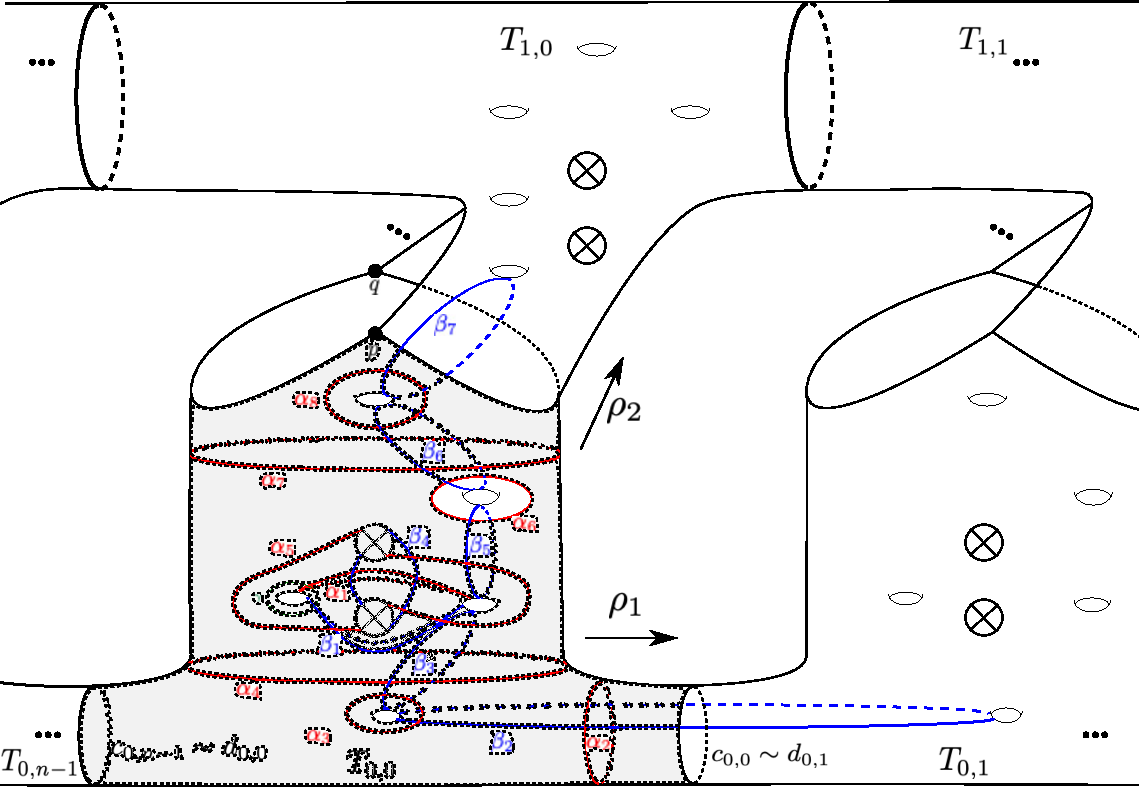
\includegraphics[scale=0.6]{surfaces1}
    \caption{Part of surface $P_{n,k}$ that includes the subsurface $T_{0,0}$ and the curves $\alpha_i$, $\beta_j$, and $\gamma$.}
    \label{fig:curves}
\end{figure}



Let $\{\alpha_1,\cdots,\alpha_8\}$ be the multi-curve in $T_{0,0}$ as shown in \autoref{fig:curves}.  Let $\{\beta_1,\cdots,\beta_7\}$ be the multi-curve in $T_{0,0}\cup T_{0,1}\cup T_{1,0}$ shown in \autoref{fig:curves}. 

For any $\alpha_i$, we choose a marking $\zeta_{\alpha_i}$ to be orientation-preserving.  For any $\beta_j$ let $\zeta_{\beta_j}$ be
orientation reversing. From here forward, we will think of $\alpha_i$ and $\beta_j$ as (inconsistently) marked curves but we will suppress the marking maps. These choices give an inconsistent marking of $\{\alpha_1,\cdots,\alpha_8\}\cup\{\beta_1,\cdots,\beta_7\}$.

Let
$$\mathcal{R}=\displaystyle\bigcup_{i=2}^8\alpha_i.$$ Then $\mathcal{R}$ is a marked multi-curve that is disjoint from $\gamma$.  Let
$$\overline{\mathcal{R}}= \mathcal{R} \cup \rho_1(\mathcal{R}) \cup \dots \cup
\rho_1^{n-1}(\mathcal{R}).$$
Let $\Phi_r$ be the composition of Dehn twists about the marked curves in $\overline{\mathcal{R}}$.  Because the curves in $\overline{\mathcal{R}}$ are disjoint, the Dehn twists about the curves commute.

Let $$\mathcal{B}=\displaystyle\bigcup_{j=2}^7\beta_j$$ in $T_{0,0} \cup T_{0,1} \cup T_{1,0}$. As above, $\mathcal{B}$ is a marked multi-curve that is disjoint from $\gamma$.  Let $$\overline{\mathcal{B}} = \mathcal{B} \cup \rho_1(\mathcal{B}) \cup \dots \cup
\rho_1^{n-1}(\mathcal{B}).$$
Let $\Phi_b$
as the composition of Dehn twists about all of the marked curves in $\overline{\mathcal{B}}$.
As with $\overline{\mathcal{R}}$, the Dehn twists about curves in $\overline{\mathcal{B}}$
commute.




Let $\alpha_1,\beta_1 \subset T_{0,0}$ be the (marked) curves in \autoref{fig:curves}. Let $\Phi$ be the composition
of Dehn twists along all the curves $\alpha_1, \rho_1(\alpha_1), \dots, \rho_1^{n-1}(\alpha_1)$ followed by
Dehn twists along all the curves $\beta_1,\rho_1(\beta_1),\dots,\rho_1^{n-1}(\beta_1)$. Define the map $f_{n,k}$
as:
\begin{align*}
    f_{n,k} &\coloneqq \rho_2 \circ \Phi \circ \Phi_b \circ \Phi_r
\end{align*}
Since the curves about which we twist to construct $f_{n,k}$ satisfy the conditions of Penner's construction, $f_{n,k}$ is a pseudo-Anosov homeomorphism.

\p{Step 3: Bounding the Stretch Factor}
Following Yazdi, our next goal is to find an upper bound for the stretch factor of the pseudo-Anosov homeomorphisms $f_{n,k}$.


\p{Train tracks} Let $S$ be a surface.  A \textit{train track} in $S$ is graph embedded in $S$ with that property that for every vertex $v$ of valence three or greater, all edges adjacent to $v$ have the same tangent vector at $v$. Let $\varphi:S\rightarrow S$ be a pseudo-Anosov homeomorphism.  The map $\varphi$ is equipped with a train track whose image under $\varphi$ is homotopic to itself.  Such a train track is an \textit{invariant train track} associated to $\varphi$. Invariant train tracks have an associated matrix whose Perron-Frobenius eigenvalue is the stretch factor of $\varphi$.


Yazdi uses the Lemma \ref{lem:spectral} to bound the spectral radius of the associated matrices.

\begin{lem}[Lemma 2.3 of \cite{yazdi2018pseudo}]
\label{lem:spectral}
Let $A$ be a non-negative integral matrix, $\Gamma$ be the adjacency graph of $A$, and $V(\Gamma)$ the set of
vertices of $\Gamma$. For each $v \in V(\Gamma)$, define $v^+$ to be the set of vertices $u\in V(\Gamma)$ such that there
is an oriented edge from $v$ to $u$. Let $D$ and $k$ be fixed natural numbers. Assume the following conditions
hold for $\Gamma$:
\begin{enumerate}[(i)]
\item For each $v \in V(\Gamma)$ we have $\deg_{\text{out}}(v) \leq D$,
\item There is a partition $V(\Gamma) = V_1 \cup \dots \cup V_\ell$ such that for each $v \in V_i$ we have
  $v^+ \subset V_{i+1}$, for any $1 \leq i \leq \ell$ except possibly when $i = 1$ or 3 (indices are mod $\ell$),
\item For each $v \in V_1$, we have $v^+ \subset V_2 \cup V_3$,
\item For each $v \in V_3$ we have $v^+ \subset V_3 \cup V_4$, and for $u \in v^+ \cap V_3$ we have
  $u^+ \subset V_4$, and
\item For all $3 < j \leq k$ and each $v \in V_j$, the set $v^+$ consists of a single element.
\end{enumerate}

Then the spectral radius of $A^{\ell-1}$ is at most $4D^4$.

\end{lem}
\noindent With this result in hand, we can find an upper bound for the stretch factor of $f_{n,k}$

\begin{lem}\label{lem:upperbound}
  Let $\lambda_{n,k}$ be the stretch factor of $f_{n,k}$. Then there exists a universal positive constant $C'$ such that for every $n \geq 1$ and $k \geq 3$, we have the following upper bound:
  \begin{align*}
   \log(\lambda_{n,k}) \leq C'\frac{n}{g_{n,k}}.
  \end{align*}
\end{lem}

\begin{proof}
 We deliberately constructed our curves so that all intersections of the multi-curve $\{\alpha_1,\dots,\alpha_8\}$ and $\{\beta_1,\dots,\beta_7\}$ occur in the subsurface $T_{0,0}$. The curve $\beta_3$ intersects $\rho_2(\alpha_3)$ at one point in $T_{0,1}$ and $\beta_7$ intersects $\rho_1(\alpha_8)$ at one point in $T_{1,0}$.

  We define the following unions of marked curves:
\begin{align*}
  \mathcal{A} &\coloneqq \mathcal{B} \cup \mathcal{R} \cup \{\alpha_1,\beta_1\} =\bigcup_{i=1}^8\alpha_i\cup\bigcup_{j=1}^7\beta_j\\
  \smallskip
  \overline{\mathcal{A}} &\coloneqq \mathcal{A} \cup \rho_1(\mathcal{A}) \cup \dots \cup \rho_1^{n-1}(\mathcal{A}) \\
  \widehat{\mathcal{A}} &\coloneqq \overline{\mathcal{A}} \cup \rho_2\left(\overline{\mathcal{A}}\right) \cup \dots \cup \rho_2^{k-1}\left(\overline{\mathcal{A}}\right).
\end{align*}

Because $f_{n,k}$ is pseudo-Anosov, it has a corresponding invariant train track $\tau$.
Let $V_{\tau}$ be the space of all measured foliations that can be obtained by varying the weights on the tracks of $\tau$.
This forms a finite dimensional cone of measures, all of which can be carried by the combinatorial train track $\tau$.
Furthermore, $f_{n,k}$ acts linearly on this cone, and leaves the cone invariant, since $\tau$ is an invariant track for $f_{n,k}$.
Consider now the transverse measure $\mu_{\delta}$ for any curve $\delta$ in $\widehat{\mathcal{A}}$.
This transverse measure is carried by $\tau$, and thus $\mu_{\delta}$ belongs in the cone of measures $V_{\tau}$.
Let $H$ be the subspace spanned by $\{\mu_\delta \mid \delta\subset\widehat{\mathcal{A}}\}$.
This linear subspace is also left invariant by $f_{n,k}$.  Let $M$
be the matrix representing the linear action of $f_{n,k}$ on $H$ with respect to the basis $\{\mu_\delta \mid \delta\subset\widehat{\mathcal{A}}\}$.  Let $\Gamma$ be the adjacency graph for $M$. Work of Penner \cite{penner1988construction} tells us that the Perron--Frobenius eigenvalue of $M$ is the stretch factor of $f_{n,k}$.


To bound the spectral radius of $M$, we need to show that $\Gamma$ satisfies
the criteria of Lemma \ref{lem:spectral}.



\begin{enumerate}[(i)]
\item There exists a constant $D'$, independent of $n$ and $k$, such that for every curve $\delta \in \widehat{\mathcal{A}}$, the geometric
  intersection number between $\delta$ and every curve in $\overline{\mathcal{A}}$ is at most $D'$.  %Recall from \autoref{sec:backgr-mapp-class} that we refer to the linear action of $f_{n,k}$ on the subspace of the cone of transverse measures on our invariant train track corresponding to connected curves in $\widehat{\mathcal{A}}$ as $M$.
  Recall that $f_{n,k}=\rho_2\circ\Phi\circ\Phi_b\circ\Phi_r$.  Let $M_1,M_2,M_3$ and $M_4$ be the matrices describing the linear action of $\Phi_r,\,\Phi_b,\,\Phi$ and $\rho_2$ on $H$, respectively. The matrix
  $M$ can then be written as a product:
  \begin{align*}
    M = M_4M_3M_2M_1.
  \end{align*}
  For a curve $\delta \in \widehat{\mathcal{A}}$, the $L^1$-norm of $M_i(\mu_\delta)$ is bounded above by the geometric intersection of
  $f_{n,k}(\delta)$ with the curves in $\overline{\mathcal{A}}$.  Thus each of $M_1$, $M_2$, and $M_3$ will change the norm by
  a factor of at most $(1 + D')$. Since $\rho_2$ will not change intersection numbers, $M_4$ will preserve the
  $L^1$-norm. If we let $D = (1 + D')^3$, then the outward degree of each vertex in $\Gamma$ is at most $D$.

\medskip
For the remaining conditions, we partition the vertices of $\Gamma$.  Observe
$$\widehat{\mathcal{A}} = \rho_{2}^{-1}(\overline{\mathcal{A}})\cup\overline{\mathcal{A}}\cup\bigcup_{i=3}^k \rho_2^{i-2}(\overline{\mathcal{A}}).$$ Then define $V_1$ as the vertices of $\Gamma$ corresponding to $\rho_2^{-1}(\overline{\mathcal{A}})$, the set $V_2$ as the vertices of $\Gamma$ corresponding to $\overline{\mathcal{A}}$, and $V_i$ for
$3 \leq i \leq k$ as the vertices of $\Gamma$ corresponding to elements in
$\rho_2^{i-2}(\overline{\mathcal{A}})$.
\item Suppose that $v \in V_i$ for $i \neq 1,3$, is a vertex
  that corresponds to $\mu_\delta$ for a curve $\delta \in \widehat{\mathcal{A}}$.  % Then $\delta$ must be a curve in $\rho_2^{i-2}(\overline{\mathcal{A}})$, for $i \neq 1,3$.
  Then $\delta$ is disjoint from all curves in $\overline{\mathcal{A}}$.  The action of $\Phi\circ\Phi_b\circ\Phi_r$ on $\widehat{\mathcal{A}}$ will preserve the set $\rho_2^{(i-2)\mod k}(\overline{\mathcal{A}})$ for each $i\neq 1,3$.  In particular, $\{\mu_\delta \mid \delta\subset\widehat{\mathcal{A}}\}$ will also be in $\rho_2^{(i-2)\mod k}(\overline{\mathcal{A}})$.  %Therefore the action of $\phi\circ\phi_b\circ\phi_r$ on $H$ will send $\mu_\gamma$ to a sum of $\mu_\eta$ where $\eta$ corresponds to elements of $V_i$.
  Then $\rho_2$ will rotate the curve $\Phi\circ \Phi_b\circ\Phi_r(\delta)$ into the set $\rho_2^{(i-1)\mod k}(\overline{\mathcal{A}})$. That is: $f_{n,k}=\rho_2\circ\Phi\circ\Phi_b\circ\Phi_r$ maps $\mu_\delta\in H$ to $$\sum_{\zeta\in \mathcal{Z}}\mu_\zeta$$ where $\mathcal{Z}$ is a subset of $\rho_2^{(i-1)\mod k}(\overline{\mathcal{A}})$.  Therefore $f_{n,k}$ maps $v$ to a subset of $V_{i+1}$.
\item To verify the third condition, we first look at the vertices $v \in V_1$ such that $v^+ \not\subset V_2$. Such vertices will correspond to the curves in $\rho_2^{-1}(\overline{\mathcal{A}})$ that $\Phi\circ\Phi_b\circ\Phi_r$ maps to curves that are not in $\rho_2(\overline{\mathcal{A}})$.  Because $\rho_1$ and $\rho_2$ commute, we can write the curves of $\rho_2^{-1}(\overline{\mathcal{A}})$ as:
    $$\rho_2^{-1}(\overline{\mathcal{A}})=\rho_2^{-1}(\mathcal{A})\cup\rho_1(\rho_2^{-1}(\mathcal{A}))\cup\cdots\cup\rho_1^{n-1}(\rho_2^{-1}(\mathcal{A})).$$  The elements of $v^+$ that are not in $V_2$ correspond to the images of curves in $\rho_2^{-1}(\overline{\mathcal{A}})$ under $f_{n,k}$ that are not in $\overline{\mathcal{A}}$.
As in Yazdi, the only curves in $\rho_2^{-1}(\overline{\mathcal{A}})$ that intersect curves in $\overline{\mathcal{A}}$ are those in the set:
\begin{align*}
    \mathcal{X} = \{ \rho_1^i(\rho_2^{-1}(\beta_7))\,\mid\,0\leq i\leq n-1\}.
  \end{align*}
  Therefore $\Phi\circ\Phi_b\circ\Phi_r$ maps curves in $\mathcal{X}$ to curves in $\rho_2^{-1}(\overline{\mathcal{A}})\cup\overline{\mathcal{A}}$.  Then $f_{n,k}=\rho_2\circ\Phi\circ\Phi_b\circ\Phi_r$ maps curves in $\mathcal{X}$ to curves in $\overline{\mathcal{A}}\cup\rho_2(\overline{\mathcal{A}}).$  
For any curve in $\mathcal{X}$, the corresponding vertex $v\in V_1$ will have
  $v^+ \subset V_2 \cup V_3.$  Moreover, $f_{n,k}$ maps the curves $\rho_2^{-1}(\overline{\mathcal{A}})\setminus \mathcal{X}$ to curves in $\overline{\mathcal{A}}$.  Thus for any vertex $v\in V_1$ that does not correspond to an element of $\mathcal{X}$, the set $v^+$ is contained in $V_2$.
\item  Similarly, we look for the $v \in V_3$ such that $v^+ \not\subset V_4$.  Such vertices will correspond to the curves in $\rho_2(\overline{\mathcal{A}})$ that $\Phi\circ\Phi_b\circ\Phi_r$ maps to curves that are not in $\rho_2^2(\overline{\mathcal{A}})$.  As above, we have: $$\rho_2(\overline{\mathcal{A}})=\rho_2(\mathcal{A})\cup\rho_1(\rho_2(\mathcal{A}))\cup\cdots\cup\rho_1^{n-1}(\rho_2(\mathcal{A})).$$
The elements of $v^+$ that are not in $V_4$ correspond to the the images of $\rho_2(\overline{\mathcal{A}})$ that intersect the curves in $\overline{\mathcal{A}}$.
The only vertices of $V_4$ that correspond to such curves are those in the set:
 $$\mathcal{Y}=\{\rho_1^i(\rho_2(\alpha_8))\,\mid\,0\leq i\leq n-1\}.$$ %The set $\mathcal{Y}$ consists of the curves corresponding to vertices of $V_3$ that intersect with the curves in $\overline{\mathcal{A}}$, namely the curves $\rho_1^i(\beta_8)$.



  For any element $v \in V_3$ corresponding to a curve in $\mathcal{Y}$ and any
  $u \in v^+ \cap V_3$, the vertex $u$ does not correspond to an element of $\mathcal{Y}$.  Therefore $u^+ \subset V_4$.
\item All the curves corresponding to an element of $V_j$, $3 < j \leq k$ are disjoint from all the curves in
  $\overline{\mathcal{A}}$. Thus, $f_{n,k}$ just acts by rotation.
\end{enumerate}

Let $\lambda = \lambda_{n,k}$ be the stretch factor of $f_{n,k}$.  By Lemma \ref{lem:spectral}, we have:
\begin{gather*}
    \lambda^{k-1} = \rho(M)^{k-1} = \rho(M^{k-1}) \leq 4D^4.
\end{gather*}
Then the logarithm of $\lambda$ satisfies:
$$\log(\lambda^{k-1})=(k-1)\cdot \log(\lambda) \leq \log(4D^4).$$
Then for $k\geq 2$
    $$\frac{k}{2}\log(\lambda) \leq (k-1)\log(\lambda) \leq \log(4D^4).$$
On the other hand, we know $g_{n,k} = (14k - 2)n + 2 \leq 14kn$ by Lemma \ref{lem:genera}. Therefore
\begin{align*}
    \log(\lambda) \leq 2\log(4D^4)\cdot\frac{1}{k} \leq 2\log(4D^4)\cdot \frac{14n}{g_{n,k}}.
\end{align*}
Let $C' \coloneqq 28\log(4D^4)$ to complete the result.
\end{proof}

\p{Step 4: The Mapping Torus}

We have now constructed an infinite family of non-orientable surfaces $P_{n,k}$ and pseudo-Anosov homeomorphisms $f_{n,k}:P_{n,k}\to P_{n,k}$, but this is not
enough. In Lemma \ref{lem:genera}, we show that $\{P_{n,k}\}$ does not include surfaces of infinitely many genera. We use the strategy of McMullen \cite{mcmullen2000polynomial} and our extension of the Thurston's
fibered face theory to fill in the gaps. 

Next we follow the strategy of Leininger--Margalit \cite{leininger2013number} to find a surface embedded in the mapping torus of minimal genus.  In our situation, this means that we will construct an embedded surface homeomorphic to $\no_3$.


\begin{figure}[t]
    \centering
    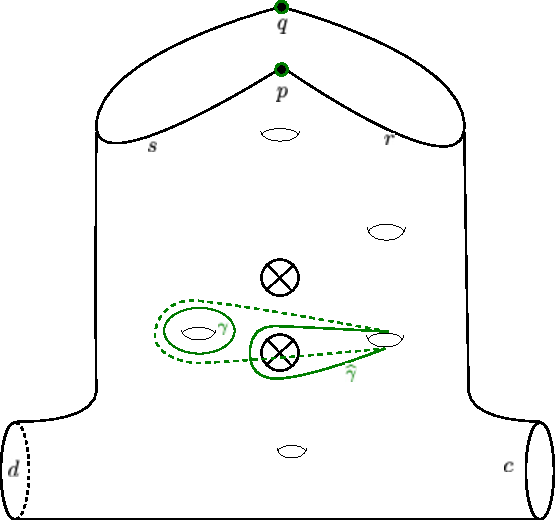
\includegraphics[scale=0.75]{gamma}
    \caption{The curves $\gamma$ and $\widehat{\gamma}$ bound an a non-orientable surface of genus 1.}
    \label{fig:gammacurves}
\end{figure}

\begin{prop}
\label{lem:genus3}
Let $M_{n,k}$ be the mapping torus of $f_{n,k}$. Let $\mathcal{K}_{n,k}$ denote the fibered cone of
$H^1(M_{n,k};\mathbb{R})$ corresponding to the map $f_{n,k}$.
There is a relatively orientable incompressible surface $F_{n,k}$ embedded in $M_{n,k}$ that is homeomorphic to $\mathcal{N}_3$.
Moreover $F_{n,k}$ is transverse to the suspension flow direction given by $f_{n,k}$ and the Poincar\'e dual of $F_{n,k}$ is in
the closure $\overline{\mathcal{K}_{n,k}}$.
\end{prop}
\begin{proof}
  Let $\gamma \subset T_{0,0}$ be the curve shown in \autoref{fig:gammacurves}. Note that $\gamma$ and $\Phi(\gamma)$ bound a non-orientable surface
  $\widehat{F}$ of genus 1 with boundary. For convenience, we will denote $\Phi(\gamma)$ by $\widehat{\gamma}$. We are going to follow the image of $\gamma$
  under powers of $f_{n,k}$.  Then we attach annuli to the
  boundary of $\widehat{F}$ to obtain $\mathcal{N}_3$. Since $\gamma$ is disjoint from all curves in $\overline{\mathcal{R}}$ and $\overline{\mathcal{B}}$ (as seen in \autoref{fig:curves}), the maps $\Phi_r$ and $\Phi_b$ act trivially on $\gamma$.  Recalling that $f_{n,k}=\rho_2\circ\Phi\circ\Phi_b\circ\Phi_r$, we have the following:
  \begin{align*}
    f_{n,k}(\gamma) &= \rho_2 \circ \Phi \circ \Phi_b \circ \Phi_r(\gamma) \\
                    &= \rho_2 \circ \Phi(\gamma) \\
                    &= \rho_2(\widehat{\gamma}) 
  \end{align*}
  It follows that for all $1\leq i\leq k$, the curve $f_{n,k}^i(\gamma)$ is $\rho_2^i(\widehat{\gamma})$.
  For $1\leq i\leq k$, let $A_i$ be an annulus in $M_{n,k}$ that connects $f_{n,k}^{i-1}(\gamma)$ to $f_{n,k}^i(\gamma)$ obtained by following the suspension
  flow of $f_{n,k}$ around $M_{n,k}$. Let $A$ be the union of all of the $A_i$, which is also an annulus.  We can now construct the embedded surface $F_{n,k}$ by taking the union of
  $A$ and $\widehat{F}$. The union of $\widehat{F}$ with $A$ has empty boundary and Euler characteristic 0, so $F_{n,k}$ is homeomorphic to $\mathcal{N}_3$.

 % The resulting surface is an embedded non-orientable surface in a non-orientable $3$-manifold, so we have
 % relative orientability by Proposition \ref{prop:relative-orientability}.

  We now need to show that $F_{n,k}$ is relatively orientable. We construct a outwards pointing normal vector field by combining the outwards pointing vector fields on $\widehat{F}$ and $A$ given by following $\gamma$ along the suspension flow.  Let $v_1$ be a vector field on $\widehat{F}$ pointing in the flow direction.  Define $v_2$ to be a vector field on $A$ as follows: on $\gamma$ define $v_2$ to be the vector field pointing in to $\widehat{F}$.  Flow the vector field along the suspension flow so $v_2$ is pointing away from $\widehat{F}$ on $\widehat{\gamma}$.
  
Let $U$ be a neighborhood of $\gamma$ in $F_{n,k}=\widehat{F}\cup A$. Define two bump functions $c_1$ and $c_2$ supported in $U$.  Let $c_1$ be $1$ on $\partial U\cap A$ and $0$ on $\widehat{F}$. Let $c_2$ be $1$ on $\partial U\cap \widehat{F}$ and $0$ on $A$.
  We add the vector fields $v_1$ on $\widehat{F}$ and $v_2$ on $A$ using these bump functions: the resulting vector field is $c_1 v_1 + c_2 v_2$.
 % Because of the way we defined the bump functions, this combined vector field agrees with both the vector fields outside of the support $U$ of the bump functions.
  Observe that since $v_1$ points in the flow direction, and $v_2$ points into the surface, the new vector field $c_1 v_1 + c_2 v_2$ is transverse, in the neighborhood of $\gamma$, to $F_{n,k}$ (see \autoref{fig:gluing-normal-field} for a picture of the resulting transverse vector field).

  We perform a similar construction in a small neighborhood of $\widehat{\gamma}$: in this case, the fact that the vector field on $\widehat{F}$ points in the flow direction, and the vector field on $A$ points away from the surface $\widehat{F}$ ensures that the new vector field is transverse, in a neighborhood of $\widehat{\gamma}$, to the surface $F_{n,k}$.

  A key fact we use in this construction is that the vector field along $A$ that starts pointing into $\widehat{F}$ at $\gamma$ comes back pointing away from the surface at $\widehat{\gamma}$: this is because the homeomorphism $f_{n,kj}$ maps the inner tubular neighborhood of $\gamma$ to the outer tubular neighborhood of $\widehat{\gamma}$, where inner and outer tubular neighborhood are the half tubular neighborhoods contained in $\widehat{F}$ and the complement respectively.
  This fact about $f_{n,k}$ follows from its definition, i.e. following the four homeomorphisms whose composition is $f_{n,k}$.
\begin{figure}[t]
  \centering
  \incfig[0.5]{gluing-normal-field}
  \caption{The left side shows the vector fields $v_1$ on $\widehat{F}$ and $v_2$ on $A$.  The upper picture is a neighborhood of $\gamma$ and the lower picture is a neighborhood of $\widehat{\gamma}$.  The right side shows the vector fields $c_1v_1+c_2v_2$ on neighborhoods of $\gamma$ and $\widehat{\gamma}$.}
  \label{fig:gluing-normal-field}
\end{figure}


  The proof that $F_{n,k}$ can be isotoped to be transverse to the suspension flow is the same as the
  proof Yazdi uses \cite{yazdi2018pseudo}, which is a restatement of that of Leininger--Margalit \cite{leininger2013number}. We include it here for completeness.

  Let $N(\gamma)$ be a tubular neighborhood of $\gamma$ in $\widehat{F}$.  Let $\eta: \widehat{F} \xrightarrow{} [0,1]$ be a smooth function supported on $N(\gamma)$ with the following properties:
  \begin{itemize}
      \item $\eta^{-1}(1) = \gamma$ and
      \item the derivative of $\eta$ vanishes on $\gamma$.
    \end{itemize}
Let $\pi:M_{n,k}\rightarrow S^1$ be the projection map and let $t_0$ be such that $\widehat{F}\subset\pi^{-1}(t_0)$.  Let $g: \widehat{F} \xrightarrow{} M_{n,k}$ be the suspension flow of $f_{n,k}$ defined as $g(x) =(x,t_0+k\cdot\eta(x))$. Then the restriction of $g$ to the interior of $\widehat{F}$ is an embedding into $M_{n,k}$ and $g(\gamma) = \widehat{\gamma}$. Therefore the image of $\widehat{F}$ under $g$ is an embedded non-orientable surface of genus three. Moreover, $g(\widehat{F})$ is isotopic to the natural embedding of $F_{n,k}$ in $M_{n,k}$, and is transverse to the suspension flow.
  Therefore, the Poincar\'e dual of $F_{n,k}$ is in $\overline{\mathcal{K}_{n,k}}$ by \autoref{thm:classifying-fibrations}.

  Finally, $F_{n,k}$ is incompressible in $M_{n,k}$ because $M_{n,k}$ is hyperbolic, and $F_{n,k}$ is genus $3$, the
  lowest possible genus for a hyperbolic non-orientable surface.
\end{proof}



\p{Step 5: Filling in the Gaps}
Recall that the family of surfaces $P_{n,k}$ that we have constructed have genera in the set $\{(14k-2)n+2\}$.
We now want to construct surfaces of genera not in the set $\{(14k-2)n+2\}$ and pseudo-Anosov homeomorphisms of those surfaces that have small stretch factors.  To do this we use the mapping torus $M_{n,k}$ of $P_{n,k}$ by $f_{n,k}:P_{n,k}\to P_{n,k}$. By Proposition \ref{lem:genus3}, there exists a relatively incompressible surface $F_{n,k}$ in $M_{n,k}$ that is homeomorphic to $\no_3$.  Let $P_{n,k}^r$ be the oriented sum of $P_{n,k}$ and
$rF_{n,k}$, as defined in Proposition $\ref{thm:oriented-sum}$.  The surfaces $P_{n,k}^r$ will be surfaces of the remaining genera.

\begin{lem}
  The surface $P^r_{n,k}$ is of genus $g^r_{n,k} = g_{n,k} + r$. In particular, as $r$ varies between
  $0$ and $14n$, the genera of $\{P^r_{n,k}\}$ spans the range between $g_{n,k}$ and $g_{n,k+1}$. Moreover,
  $P^r_{n,k}$ is isotopic to a fiber of a fibration of $M_{n,k}$ with pseudo-Anosov monodromy that fixes $2n$
  of the singularities of its invariant foliation.
\end{lem}

\begin{proof}
  The Euler characteristic of an oriented sum is the sum of the Euler characteristics of the summands:
  \begin{align*}
    \chi(P^r_{n,k}) &= \chi(P_{n,k}) + r\cdot\chi(F_{n,k}) \\
                    &= (-2g_{n,k} + 2)-2r \\
                    &= -2(g_{n,k} + r) + 2.
  \end{align*}
  Since $P_{n,k}^r$ has no boundary or punctures, we have that the genus of $P_{n,k}^r$ is $g_{n,k}+r$.

  By Lemma \ref{lem:genus3} we know that $F_{n,k}$ is incompressible and transverse to the suspension flow given by $f_{n,k}$.  Therefore by Proposition \ref{prop:asymptotic}, there is a pseudo-Anosov homeomorphism $f_{n,k}^r$ of $P_{n,k}^r=P_{n,k}+rF_{n,k}$.
  

 As in Yazdi \cite[Lemma 3.5]{yazdibounds}, $f_{n,k}$ fixes the $2n$ singularities of the stable foliation that are the intersection points of the axis of $\rho_1$ with
  $P_{n,k}$. By Lemma \ref{lem:genus3}, the surface $F_{n,k}$ can be isotoped to be transverse to
  the suspension flow and disjoint from the orbit of the $2n$ singularities of $f_{n,k}$.  Hence the monodromy
  $f^r_{n,k}$ still fixes the corresponding $2n$ singularities on $P^r_{n,k}$.
\end{proof}

We now prove the non-orientable version of the final piece of Yazdi's proof \cite[Lemma 3.6]{yazdi2018pseudo}.
\begin{lem}
\label{lem:bound}
Let $\lambda_{n,k}^r$ be the stretch factor of $f_{n,k}^r:P_{n,k}^r\rightarrow P_{n,k}^r$. Then there exists a constant $C > 0$ such that for every $n \geq 1$, $k \geq 3$, and $0 \leq r \leq 14n$ we have the following upper bound on $\log(\lambda_{n,k}^r)$:
\begin{align*}
  \log(\lambda^r_{n,k}) \leq C\frac{n}{g^r_{n,k}}.
\end{align*}
\end{lem}
\begin{proof}
  Let $\mathcal{K} = \mathcal{K}_{n,k}$ be the fibered cone in $H^1(M_{n,k};\mathbb{R})$ corresponding to $f_{n,k}$ and $h: \mathcal{K} \xrightarrow[]{} \mathbb{R}$
  the function described in \autoref{thm:fm}. Note that $g_{n,k}\geq 42$, therefore we have the following bounds on $g_{n,k}^r$:
  \begin{align*}
    g^r_{n,k} &= g_{n,k} + r \\
              &\leq g_{n,k} + 14n \\
              &< 2g_{n,k}.
  \end{align*}
  Let $\omega$ be the Poincar\'e dual of $P^r_{n,k}$ and $\alpha$ the Poincar\'e dual of $P_{n,k}$.  Then the following string of inequalities holds:
  \begin{align*}
    h([\omega]) &< h([\alpha]) &&\text{(Convexity of $h$)}\\
                &\leq C'\frac{n}{g_{n,k}} &&\text{(Lemma \ref{lem:upperbound})}\\
                &\leq 2C'\frac{n}{g^r_{n,k}}&&\text{(upper bound for $g_{n,k}^r$)}.\qedhere
  \end{align*}
\end{proof}


In the initial construction of $P_{n,k}$, there were $2n$  marked points, which were singularities of the map $f_{n,k}$.  By the construction of $P_{n,k}^r$, these marked points are also singularities of $f^r_{n,k}$.  Now we puncture $P_{n,k}^r$ at $n$ of these marked points.  We could think of this as removing all copies of the point $p$ in the construction of $P_{n,k}$ in step 1. %as a map on a non-orientable surface of genus $g^r_{n,k}$ with $n$ punctures. Also note from above weknow $g^r_{n,k}$ covers all natural numbers between $g_{n,k}$ and $g_{n,k+1}$, thus this set of genera for all $r$ covers all natural numbers larger than $g_{n,3} = 40n + 2$.

We can now give a proof of \autoref{thm:stretch1}.


\begin{proof}[Proof of \autoref{thm:stretch1}]
As above, the lower bound follows easily from the lower bound in the orientable setting.  

  To find the upper bound, let $C'=\frac{C}{2}$ be the value given in Lemma \ref{lem:bound}. Let $B'_2(n)$ be the
  following quantity:
  \begin{align*}
    B'_2(n) = \max\{2C'n, \ell'_{1,n}, 2\ell'_{2,n}, \dots, (40n + 1)\ell'_{40n+1,n}\}.
  \end{align*}
  By Proposition \ref{prop:asymptotic} and Lemma \ref{lem:bound}, $B'_2(n)$ is an upper bound for $g\cdot \ell'_{g,n}$.
\end{proof}